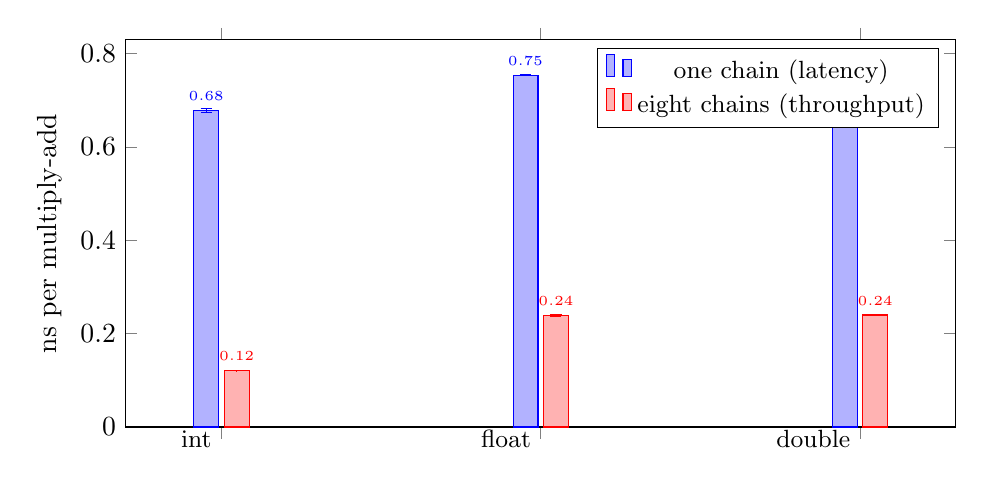
\begin{tikzpicture}
\begin{axis}[ybar, width=\textwidth, height=6.5cm, bar width=9pt, ymin=0, symbolic x coords={int,float,double}, xtick=data, x tick label style={rotate=0, anchor=east, font=\small}, ylabel={ns per multiply-add}, enlarge x limits=0.15, legend style={font=\small, at={(0.98,0.98)}, anchor=north east}, nodes near coords, nodes near coords style={font=\tiny}, every node near coord/.append style={/pgf/number format/.cd, fixed, precision=2}]
\addplot+[error bars/.cd, y dir=both, y explicit] coordinates {(int,0.6785) +- (0,0.0042) (float,0.7531) +- (0,0.0010) (double,0.7521) +- (0,0.0018)};
\addlegendentry{one chain (latency)}
\addplot+[error bars/.cd, y dir=both, y explicit] coordinates {(int,0.1210) +- (0,0.0004) (float,0.2393) +- (0,0.0021) (double,0.2400) +- (0,0.0010)};
\addlegendentry{eight chains (throughput)}
\end{axis}
\end{tikzpicture}